\documentclass{article}

\PassOptionsToPackage{numbers,compress}{natbib}
\usepackage[dblblindworkshop]{neurips_2026}
\workshoptitle{7th Muslims in Machine Learning Workshop (MusIML), NeurIPS 2026}

\usepackage{amsmath,amssymb,amsfonts}
\usepackage{booktabs}
\usepackage{multirow}
\usepackage{array}
\usepackage{microtype}
\usepackage{url}
\usepackage{hyperref}
\usepackage{graphicx}
\usepackage{float}
\usepackage[utf8]{inputenc}
\usepackage[T1]{fontenc}
\hypersetup{colorlinks=false,hidelinks}
\setlength{\textfloatsep}{8pt plus 2pt minus 2pt}
\setlength{\floatsep}{7pt plus 2pt minus 2pt}
\setlength{\intextsep}{7pt plus 2pt minus 2pt}

\title{Nomenclature and Context Sensitivity of Zero-Shot Biological Vision--Language Models for Bangladeshi Freshwater Fish Recognition}
\author{Anonymous Author(s)}
% Camera-ready example (enable only if the portal requests author-visible PDF):
% \author{First Author \quad Second Author \quad Third Author \\
% Institution / Department \\
% City, Country \\
% \texttt{contact@example.edu}}

\begin{document}
\maketitle

\begin{abstract}
Zero-shot vision--language models (VLMs) are increasingly used as training-free species recognizers, but reported accuracy can reflect more than visual species knowledge. We audit CLIP, BioCLIP, BioCLIP2, and a multilingual Jina CLIP v2 control on seven freshwater-fish categories from two Bangladeshi sources (10,321 images). BioCLIP2 reaches 72.36\% on BFF-15 with English common names and 68.91\% on SylFishBD with scientific names, versus 25.15\% and 14.40\% for generic CLIP. BioCLIP2 Bengali prompts are near chance in balanced accuracy (14.22--14.29\%); Jina partially recovers Bengali discrimination to 21.89\% and 16.36\%, but bare Bengali names return to 14.29\% on both sources. Paired SylFishBD interventions show no significant weak-blur effect, modest losses from stronger blur/gray masking, a larger white-mask artifact, and strong species dependence. Zero-shot biological VLM scores therefore jointly reflect biological specialization, multilingual alignment, nomenclature, prompt formulation, and context.
\end{abstract}

\section{Introduction}
Automated species recognition supports biodiversity monitoring, fisheries, aquaculture, and market inspection. Fish recognition is difficult because related taxa may differ subtly while pose, illumination, occlusion, and background vary. Conventional systems therefore rely on labeled data and supervised transfer learning \citep{shah2019fishpak,xu2021seresnet,das2024bdfreshwater}, but high in-domain accuracy does not establish transferable biological knowledge.

Contrastive vision--language pre-training offers a training-free alternative. CLIP enables zero-shot image--text classification \citep{radford2021clip}, while BioCLIP and BioCLIP2 add biologically structured pre-training for fine-grained recognition \citep{stevens2024bioclip,gu2025bioclip2}. Fish work has also explored language supervision and training-free multimodal recognition \citep{dai2024clipfssc,jose2026zeroshot}.

For VLMs, the class label is part of the classifier: small wording changes can alter CLIP predictions \citep{zhou2022coop,zhou2022cocoop}. Biology amplifies this issue because one organism may have vernacular, English-common, scientific, historical, or synonymous names; scientific binomials are not always optimal \citep{parashar2023scientific}, and multilingual VLMs show large cross-language gaps \citep{geigle2024babel,chung2026uclip}. In Bangladesh, success through English or Latin strings but failure through Bengali names can overstate local accessibility.

Visual context introduces a parallel ambiguity: classifiers can exploit backgrounds and shortcuts \citep{geirhos2020shortcut,xiao2021backgrounds}, while CLIP can retain domain-sensitive information \citep{wen2025diverse}. We therefore ask: \emph{how stable is zero-shot biological recognition when the model, language, nomenclature, prompt, or context changes?}

Our contributions are:
\begin{itemize}
  \item a cross-model, cross-source zero-shot benchmark of CLIP, BioCLIP, and BioCLIP2 on seven Bangladeshi freshwater-fish categories;
  \item a nomenclature audit spanning Romanized vernacular, Bengali script, English-common and scientific names, prompt templates, and scientific synonyms, augmented with a multilingual Jina CLIP v2 control that separates multilingual alignment from biological specialization;
  \item paired context interventions on 7,665 SylFishBD images using graded blur, neutral masks, cropping, background-only views, and cross-species background swaps, with paired inference and multiple-testing correction.
\end{itemize}

\begin{figure*}[t]
\centering
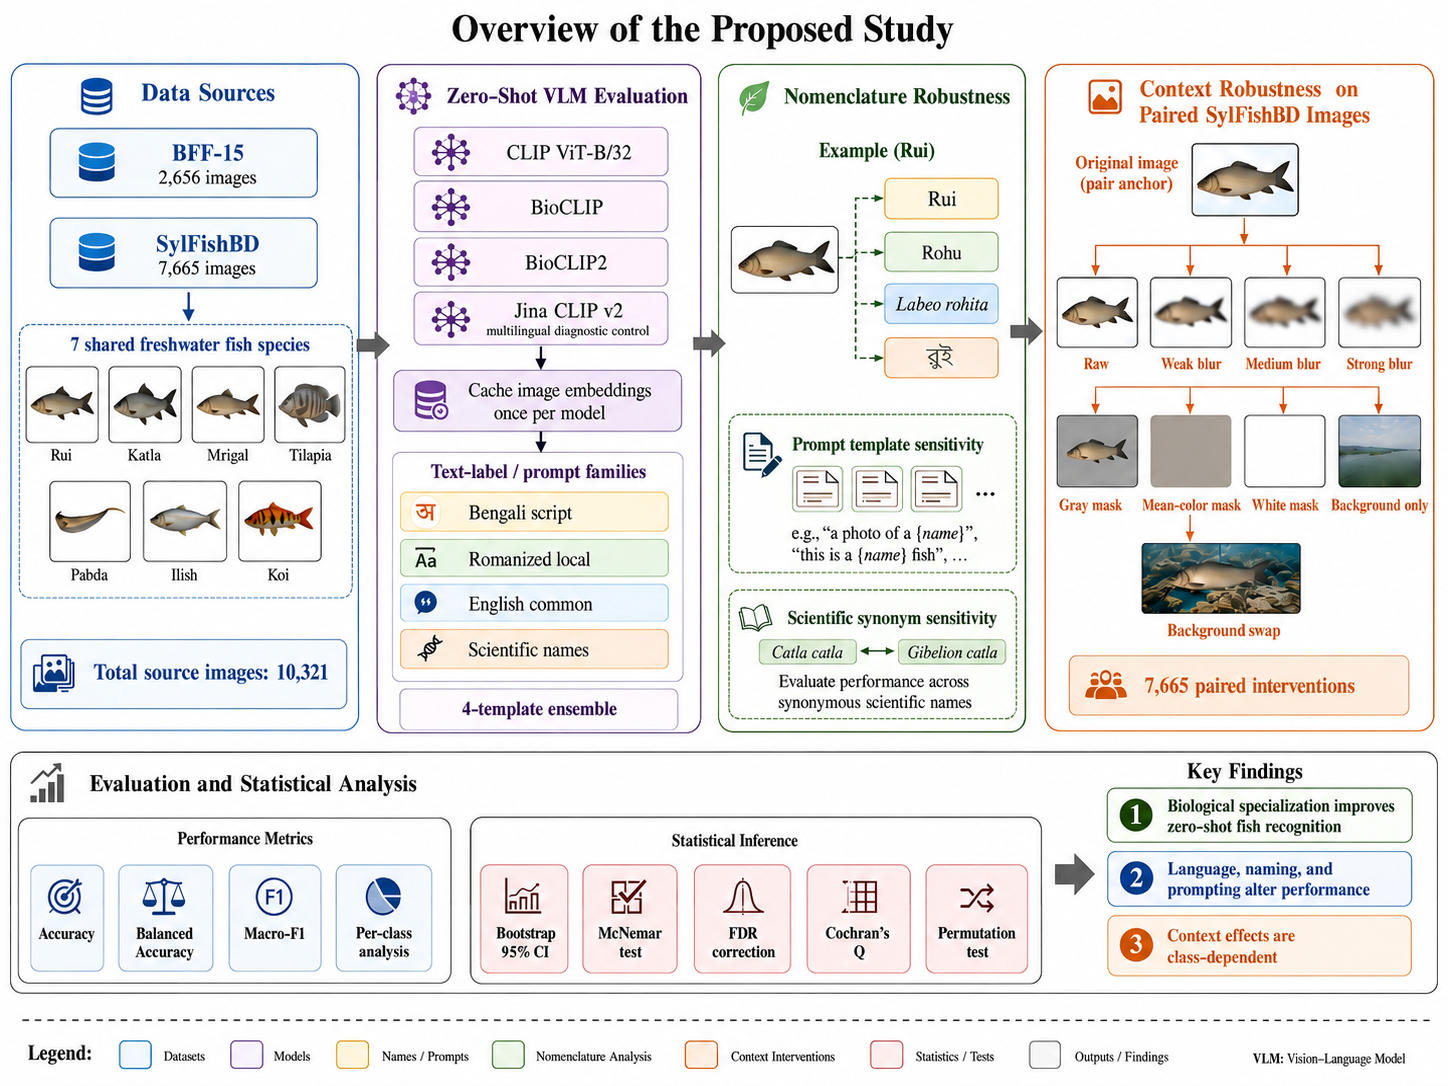
\includegraphics[width=0.97\textwidth]{overview_updated.png}
\caption{Study overview. Seven shared fish categories are evaluated with frozen CLIP, BioCLIP, and BioCLIP2; Jina CLIP v2 is a multilingual Bengali-interface control. We probe nomenclature/prompt robustness, paired context interventions, and statistical reliability.}
\label{fig:overview}
\end{figure*}

\section{Related Work}
\paragraph{Prompt and nomenclature robustness.}
CLIP generates class prototypes through language rather than fixed task weights \citep{radford2021clip}. CoOp/CoCoOp showed that prompt context changes downstream behavior \citep{zhou2022coop,zhou2022cocoop}; in species recognition, common English names can outperform scientific names \citep{parashar2023scientific}. We keep weights fixed and treat name/prompt choices as evaluation variables.

\paragraph{Biological and multilingual VLMs.}
BioCLIP and BioCLIP2 use taxonomically informed contrastive pre-training at increasing scale \citep{stevens2024bioclip,gu2025bioclip2}. Multilingual evaluation reveals a different axis of quality: Babel-ImageNet reports large cross-language variation \citep{geigle2024babel}, while uCLIP extends VLMs multilingually \citep{chung2026uclip}. We use multilingual Jina CLIP v2 \citep{koukounas2024jinaclipv2} as a Bengali-alignment control, not a biological baseline.

\paragraph{Regional fish data and context.}
Bangladesh-specific fish resources include SylFishBD with SAM-derived instance masks \citep{absar2026sylfish,kirillov2023sam} and BFF-15 \citep{bff15}. Recent self-supervised work achieves high in-domain accuracy after fine-tuning \citep{siam2025freshwater}; our models and prompts remain frozen. Background controls are motivated by evidence that context alone can retain class information \citep{xiao2021backgrounds}.

\section{Methodology}
\subsection{Data harmonization}
We use seven categories shared by BFF-15 and SylFishBD: Rui, Katla, Mrigal, Tilapia, Pabda, Ilish, and Koi. BFF-15 contributes 2,656 images and SylFishBD 7,665 (10,321 total); every selected SylFishBD image has a binary mask. Table~\ref{tab:data} gives counts/nomenclature. All models remain frozen, so no train/validation/test split is required.

SHA-256 found no exact cross-source duplicates; a 64-bit perceptual-hash search flagged 73 low-distance pairs ($\leq 6$ bits) for review. Because similar fish can yield similar hashes, we flag rather than automatically exclude them and describe the collections as two public sources, not fully independent sources.

\begin{table}[t]
\caption{Shared seven-category benchmark. SylFishBD counts refer to source images; each has a paired segmentation mask.}
\label{tab:data}
\centering
\small
\begin{tabular}{l l l l rr}
\toprule
Class & Romanized & English & Scientific & BFF & Syl \\
\midrule
Rui & Rui & Rohu & \emph{L. rohita} & 514 & 1670 \\
Katla & Katla & Catla & \emph{C. catla} & 427 & 1133 \\
Mrigal & Mrigal & Mrigal carp & \emph{C. cirrhosus} & 317 & 1293 \\
Tilapia & Tilapia & Nile tilapia & \emph{O. niloticus} & 383 & 1326 \\
Pabda & Pabda & Pabda catfish & \emph{O. pabda} & 348 & 862 \\
Ilish & Ilish & Hilsa & \emph{T. ilisha} & 233 & 789 \\
Koi & Koi & Climbing perch & \emph{A. testudineus} & 434 & 592 \\
\midrule
Total &&&& 2656 & 7665 \\
\bottomrule
\end{tabular}
\end{table}

\subsection{Frozen zero-shot classification and prompt construction}
We evaluate CLIP ViT-B/32 (OpenAI), BioCLIP, and BioCLIP2. For normalized image embedding $f_I(x)$ and class name $n_c$, we instantiate four templates---``a photo/image/photograph/specimen of $n_c$, a fish species''---normalize each text embedding, and form the normalized mean prototype
\begin{equation}
 t_c = \frac{\frac{1}{K}\sum_{k=1}^K \hat f_T(p_k(n_c))}{\left\|\frac{1}{K}\sum_{k=1}^K \hat f_T(p_k(n_c))\right\|_2}, \qquad K=4.
\end{equation}
Prediction is $\hat y=\arg\max_c f_I(x)^\top t_c$. Cached image embeddings ensure nomenclature experiments change only the text-side classifier.

We test Romanized, English-common, and scientific names, plus Bengali script for BioCLIP2. Templates are also evaluated individually. Scientific-name controls substitute \emph{Catla catla} with \emph{Gibelion catla} or \emph{Labeo catla}, and \emph{Cirrhinus cirrhosus} with \emph{C. mrigala}; these are nomenclatural variants, not claims of uniquely correct taxonomy.

\subsection{Multilingual Bengali control}
To test whether BioCLIP2's Bengali failure reflects text alignment, we add frozen Jina CLIP v2 \citep{koukounas2024jinaclipv2}. The same 10,321 images/classes use Bengali, Romanized, English-common, and scientific labels with the same four-template ensemble and a 512-dimensional Matryoshka-truncated representation; no benchmark tuning is performed.

A secondary \emph{name-only} control embeds only Bengali class names, testing whether multilingual support alone suffices or interacts with prompt framing. This directly tests whether BioCLIP2's near-chance Bengali result is partly a text-alignment limitation rather than a property of Bengali nomenclature itself. Jina is not used for context interventions; it is diagnostic for multilingual alignment versus biological specialization.

\subsection{Paired context interventions}
SylFishBD masks preserve foreground pixels while altering background. We apply Gaussian blur ($\sigma=0.01,0.03,0.06$ times the shorter dimension), white/gray/mean-color masks, a 10\%-expanded tight crop, foreground removal with Telea inpainting, and cross-species background swaps. These are stress tests, not perfect causal isolation, because synthetic transformations introduce distribution shift.

\subsection{Metrics and inference}
We report accuracy, balanced accuracy, macro-F1, and per-class effects. Class-stratified bootstrap CIs use 1,000 resamples for the primary benchmark and 2,000 for robustness/multilingual controls. Paired comparisons use exact two-sided McNemar tests and bootstrap accuracy differences with Benjamini--Hochberg FDR correction. Cochran's $Q$ tests context conditions; donor-follow uses 5,000 label permutations. Seed is 42.

\section{Results and Discussion}
\subsection{Biology-specialized VLMs outperform the tested generic CLIP baseline}
Table~\ref{tab:primary} shows a large gap between generic and biology-specialized VLMs. With scientific names, CLIP scores 15.40\%/14.40\% on BFF-15/SylFishBD, BioCLIP 47.82\%/58.88\%, and BioCLIP2 69.99\%/68.91\%. With English names BioCLIP2 reaches 72.36\%/64.59\%. Relative to BioCLIP, BioCLIP2 gains 22.18 and 10.03 points under scientific prompting (paired 95\% CIs [19.73, 24.66] and [8.91, 11.17], both $q<0.001$). Because checkpoints also differ in scale/training recipe, we do not attribute the full gap solely to specialization.

\begin{table}[t]
\caption{Primary zero-shot benchmark. Values are accuracy / macro-F1 (\%).}
\label{tab:primary}
\centering
\small
\begin{tabular}{llcc}
\toprule
Model & Prompt & BFF-15 & SylFishBD \\
\midrule
CLIP ViT-B/32 & Romanized & 10.96 / 5.64 & 16.95 / 13.15 \\
 & English & 25.15 / 20.03 & 23.80 / 22.05 \\
 & Scientific & 15.40 / 6.97 & 14.40 / 7.21 \\
\midrule
BioCLIP & Romanized & 25.26 / 18.28 & 27.93 / 16.63 \\
 & English & 54.89 / 51.61 & 52.26 / 46.64 \\
 & Scientific & 47.82 / 43.34 & 58.88 / 57.45 \\
\midrule
BioCLIP2 & Romanized & 35.77 / 25.98 & 37.56 / 25.19 \\
 & English & \textbf{72.36} / 67.33 & 64.59 / 64.30 \\
 & Scientific & 69.99 / 68.85 & \textbf{68.91} / 69.68 \\
\bottomrule
\end{tabular}
\end{table}

\subsection{Nomenclature and prompt formulation are part of the classifier}
With identical BioCLIP2 image embeddings, BFF-15 scores 35.77\%/72.36\%/69.99\% for Romanized/English/scientific names; SylFishBD scores 37.56\%/64.59\%/68.91\%. Scientific terminology is therefore not universally optimal.

Bengali prompts yield 16.27\%/7.74\% accuracy and 14.22\%/14.29\% balanced accuracy, essentially seven-class chance (14.29\%). Thus these Bengali fish-name prompts provide little discrimination for the tested BioCLIP2 text encoder.

Across four individual scientific templates, BioCLIP2 spans 56.06--77.07\% on BFF-15 and 61.44--79.71\% on SylFishBD. Replacing \emph{Catla catla} by \emph{Gibelion catla} raises SylFishBD accuracy 5.14 points ($q<0.001$), while \emph{Labeo catla} lowers it 3.46 points and lowers BFF-15 by 8.58 points. Replacing \emph{Cirrhinus cirrhosus} by \emph{C. mrigala} improves both sources by about two points. Thus ``scientific prompt'' is not fully specified without the exact string/template.

\subsection{Multilingual alignment partially recovers Bengali, but does not replace biological specialization}
Under the same four-template ensemble, Jina CLIP v2 reaches 21.89\% Bengali balanced accuracy on BFF-15 (95\% CI [20.77, 23.01]) and 16.36\% on SylFishBD ([15.64, 17.05]), versus BioCLIP2's 14.22\%/14.29\%. This descriptive control suggests that the near-chance BioCLIP2 result is partly model/interface-specific.

Recovery remains incomplete: English exceeds Bengali accuracy by 4.10 points on BFF-15 (CI [2.86, 5.35], $q<10^{-8}$) and 13.70 on SylFishBD ([12.77, 14.66], $q<10^{-98}$). Bengali and Romanized are indistinguishable on BFF-15 ($q=0.617$), while Romanized exceeds Bengali by 4.66 points on SylFishBD ($q<10^{-19}$).

Jina's English accuracy (29.41\%/23.78\%) remains far below BioCLIP2 (72.36\%/64.59\%), so multilingual alignment does not replace biological specialization. Bare Bengali names also collapse to exactly 14.29\% balanced accuracy on both sources, showing an interaction with prompt framing. Together, the controls expose a trade-off: stronger multilingual alignment can recover Bengali signal without matching BioCLIP2's fine-grained biological accuracy. We therefore interpret Jina as an interface diagnostic, not evidence about Bengali understanding in general.

\begin{table}[H]
\caption{Jina CLIP v2 multilingual control. Values are accuracy / balanced accuracy / macro-F1 (\%).}
\label{tab:jina}
\centering
\small
\begin{tabular}{lcc}
\toprule
Prompt family & BFF-15 & SylFishBD \\
\midrule
Bengali script & 25.30 / 21.89 / 16.31 & 10.08 / 16.36 / 6.04 \\
Romanized & 24.89 / 23.93 / 19.05 & 14.74 / 14.78 / 12.06 \\
English common & 29.41 / 28.43 / 17.87 & 23.78 / 18.01 / 15.62 \\
Scientific & 16.11 / 15.96 / 13.56 & 9.13 / 10.27 / 9.75 \\
\bottomrule
\end{tabular}
\end{table}

\subsection{Context sensitivity is real but intervention-dependent}
The white-mask comparison drops BioCLIP2 from 68.91\% to 60.52\% ($-8.39$ points), but the intervention ladder qualifies this effect (Table~\ref{tab:context}). Weak blur is nonsignificant ($-0.47$; CI [$-1.34$, 0.46], $q=0.347$); medium/strong blur reduce accuracy 2.18/2.87 points and gray/mean-color masking about 3.8 points (all $q<0.001$). Thus white masking adds substantial distribution shift.

\begin{table}[H]
\caption{BioCLIP2 context ladder on 7,665 paired SylFishBD images. $\Delta$ is change from raw; brackets are paired-bootstrap 95\% CIs.}
\label{tab:context}
\centering
\small
\begin{tabular}{lrrl}
\toprule
Condition & Acc. & $\Delta$ (pp) & FDR $q$ \\
\midrule
Raw & 68.91 & -- & -- \\
Weak blur & 68.44 & $-0.47$ [$-1.34$, 0.46] & 0.347 \\
Medium blur & 66.73 & $-2.18$ [$-3.11$, $-1.23$] & $<0.001$ \\
Strong blur & 66.04 & $-2.87$ [$-3.81$, $-1.94$] & $<0.001$ \\
Gray mask & 65.11 & $-3.80$ [$-4.79$, $-2.83$] & $<0.001$ \\
Mean-color mask & 65.10 & $-3.81$ [$-4.76$, $-2.81$] & $<0.001$ \\
White mask & 60.52 & $-8.39$ [$-9.56$, $-7.25$] & $<0.001$ \\
\bottomrule
\end{tabular}
\end{table}

\begin{figure}[H]
\centering
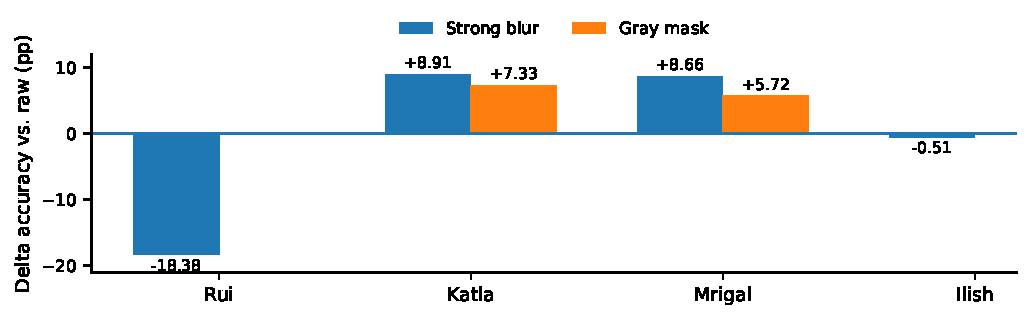
\includegraphics[width=0.76\textwidth]{context_selected_effects.pdf}
\caption{Class-conditional changes from raw SylFishBD. Strong blur helps Katla/Mrigal but sharply hurts Rui; Ilish is nearly unchanged. Gray-mask values are shown where exact effects are available.}
\label{fig:classcontext}
\end{figure}

Aggregate means conceal class dependence (Fig.~\ref{fig:classcontext}). Strong blur improves Katla/Mrigal by 8.91/8.66 points, hurts Rui by 18.38, and barely changes Ilish ($-0.51$). Gray masking shows the same heterogeneity: Katla/Mrigal improve (+7.33/+5.72), while Rui, Koi, Tilapia, and Pabda decline.

Supporting controls reject simple background-label explanations. Background-only images retain 17.90\% accuracy (21.48\% balanced; $-51.01$ points, CI [$-52.17$, $-49.84$]), confirming dominant foreground information. Cross-species swaps reduce accuracy to 56.76\% ($-12.15$; CI [$-13.24$, $-11.06$]), yet donor-follow is only 8.88\% versus a 15.10\% permutation-null mean. Tight cropping reaches 55.15\%, and five mask-geometry properties are nonsignificant after FDR ($q\ge0.097$).

\subsection{Implications and limitations}
Three implications follow. Biology-specialized VLMs outperform the tested generic CLIP baseline, although scale/training recipe also differ. Zero-shot accuracy is not an image-encoder property alone: language, exact taxonomic string, and prompt frame instantiate the classifier, as the multilingual/name-only controls demonstrate. Context robustness likewise requires a ladder of interventions rather than one synthetic mask. Practically, reporting only the best English/scientific prompt can overstate accessibility when a strong visual model exposes a weak native-language interface.

Limitations include only seven categories/two sources, unknown pre-training exposure to related imagery, one multilingual control with a 512-D truncated representation, Bengali results specific to the tested names/templates, and synonym tests limited to Katla/Mrigal. One multilingual model cannot establish a general property of multilingual VLMs. Context interventions change image distribution as well as information content, so conclusions rely on agreement across blur, masks, crop, background-only, and swap controls rather than perfect causal decomposition.

\section{Conclusion}
We audit zero-shot freshwater-fish recognition across generic, biology-specialized, and multilingual VLM interfaces. BioCLIP2 is strongest overall but remains sensitive to nomenclature, language, prompt syntax, synonyms, and context. Jina partially recovers Bengali discrimination yet is weaker at fine-grained recognition and collapses to chance with bare Bengali names. Paired context interventions show small average effects for mild degradation, larger synthetic-mask artifacts, and strong species dependence. Biological specialization and multilingual alignment address different failure modes; benchmarks should therefore report and stress-test language, exact nomenclature, prompt templates, and context.

\bibliographystyle{plainnat}
\bibliography{references}

\end{document}
